\documentclass{beamer}
\usefonttheme[onlymath]{serif}

\usepackage{amsfonts}

% Code Block Setting
\usepackage{listings}
\lstset{language=C,
numberstyle=\footnotesize,
basicstyle=\ttfamily\footnotesize,
numbers=left,
stepnumber=1,
frame=shadowbox,
breaklines=true}

\usetheme{Warsaw}
% \usecolortheme{dove}

% Add frame number and total frame number in footline
\defbeamertemplate*{footline}{shadow theme}{%
    \leavevmode%
    \hbox{\begin{beamercolorbox}[wd=.5\paperwidth,ht=2.5ex,dp=1.125ex,leftskip=.3cm plus1fil,rightskip=.3cm]{author in head/foot}%
            \usebeamerfont{author in head/foot}\hfill\insertshortauthor
        \end{beamercolorbox}%
        \begin{beamercolorbox}[wd=.4\paperwidth,ht=2.5ex,dp=1.125ex,leftskip=.3cm,rightskip=.3cm plus1fil]{title in head/foot}%
            \usebeamerfont{title in head/foot}\insertshorttitle\hfill%
        \end{beamercolorbox}%
        \begin{beamercolorbox}[wd=.1\paperwidth,ht=2.5ex,dp=1.125ex,leftskip=.3cm,rightskip=.3cm plus1fil]{title in head/foot}%
            \hfill\insertframenumber\,/\,\inserttotalframenumber
    \end{beamercolorbox}}%
    \vskip0pt%
}

% Tikz related
\usepackage{tikz}
\usetikzlibrary{fit}
\usetikzlibrary{calc}
\usetikzlibrary{positioning}

% Number the figures
\setbeamertemplate{caption}[numbered]

% Add outline page at begining of each section
\AtBeginSection[]
{
    \begin{frame}<beamer>
        \frametitle{Outline}
        \tableofcontents[currentsection, hideallsubsections]
    \end{frame}
}

%%%%%%%%%%%%%%%%%%%%%%%%%%%%%%%%%%%%%%%%%%%%%

\title{Thesis Progress report}
\author{
    Ching-Yuan, Tsai
}
\date{
    \tiny{2018,1,17}\\
    \tiny{Presented by Ching-Yuan, Tsai}
}

\begin{document}
\begin{frame}
    \titlepage
\end{frame}

\section{Introduction}

\subsection{Motivation}
\begin{frame}
    \frametitle{Motivation}
	\begin{itemize}
		\item In large module, distributed training may be slower than single-machine training. 
		\item Parameter server uses a lot of time on synchronous stage. 
		\item Network is bottleneck in our system. 
	\end{itemize}
\end{frame}


\subsection{Objective}
\begin{frame}
    \frametitle{Objective}
    \begin{itemize}
		\item Use software method to reduce network load. 
			\begin{itemize}
				\item Prune gradients by threshold. 
					\begin{itemize}
						\item static threshold
						\item standard deviation threshold
						\item dynamic threshold
					\end{itemize}
				\item Gradients request scheduling. 
			\end{itemize}
	\end{itemize}
\end{frame}



\section{Prune}

\subsection{Observation}
\begin{frame}
    \frametitle{Observation}
	\begin{figure}
		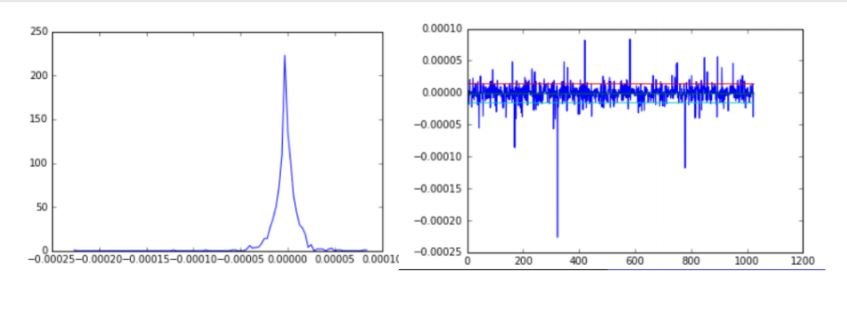
\includegraphics[scale=0.4]{figure/gradient_observation.JPG}
	\end{figure}
\end{frame}


\subsection{Prune}
\begin{frame}
    \frametitle{Prune}
    \begin{itemize}
		\item Prune gradients: Send gradients which are absolutely greater than threshold. 
			\begin{itemize}
				\item Static threshold: 10\%, 1\%, 0.1\%. 
				\item Standard deviation threshold: 1, 2, 3. 
				\item Dynamic threshold: mean of the gradients which are greater than last threshold. 
			\end{itemize}
	\end{itemize}
\end{frame}

\subsection{Standard deviation threshold}
\begin{frame}
	\frametitle{Standard deviation threshold}
	\begin{itemize}
		\item Compute standard deviation on gpu. 
		\item Faster 30 times than cpu.
		\item Use 25\% computation time. 
	\end{itemize}
\end{frame}
\begin{frame}
    \frametitle{experiment 1}
	\begin{figure}
		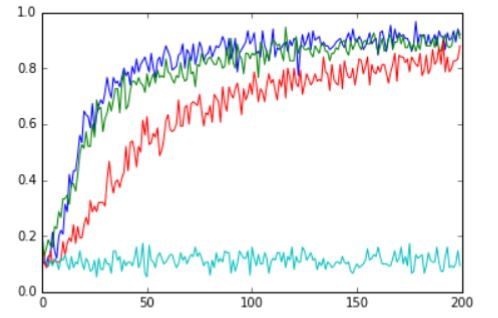
\includegraphics[scale=0.4]{figure/stdexp1.JPG}
	\end{figure}
\end{frame}

\begin{frame}
    \frametitle{experiment 2}
	\begin{itemize}
		\item To do: accuracy for each time. 
	\end{itemize}
\end{frame}

\subsection{Static threshold}
\begin{frame}
	\frametitle{Static threshold}
	\begin{itemize}
		\item Compute on gpu. 
		\item Selection algorithm. 
	\end{itemize}
\end{frame}
\begin{frame}
    \frametitle{experiment 1}
	\begin{itemize}
		\item To do: accuracy for each interation. 
	\end{itemize}
\end{frame}

\begin{frame}
    \frametitle{experiment 2}
	\begin{itemize}
		\item To do: accuracy for each time. 
	\end{itemize}
\end{frame}
\subsection{Dynamic threshold}
\begin{frame}
	\frametitle{Dynamic threshold}
	\begin{itemize}
		\item Compute on gpu. 
		\item Next threshold = mean of the gradients which are greater than current threshold
	\end{itemize}
\end{frame}
\begin{frame}
    \frametitle{experiment 1}
	\begin{itemize}
		\item To do: accuracy for each interation. 
	\end{itemize}
\end{frame}

\begin{frame}
    \frametitle{experiment 2}
	\begin{itemize}
		\item To do: accuracy for each time. 
	\end{itemize}
\end{frame}


\section{Gradients request scheduling}

\subsection{Introduction}
\begin{frame}
    \frametitle{Introduction}
	\begin{itemize}
		\item Client changes gradient request order to get some benefits.  
	\end{itemize}
\end{frame}


\subsection{Some examples}
\begin{frame}
    \frametitle{Reduce suspend}
    \begin{figure}
		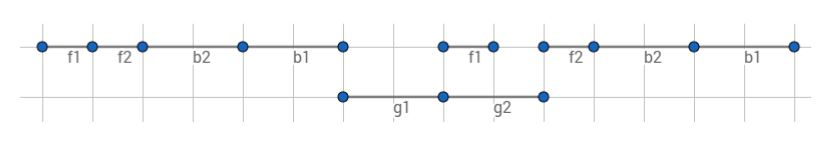
\includegraphics[scale=0.4]{figure/reducesuspend.JPG}
		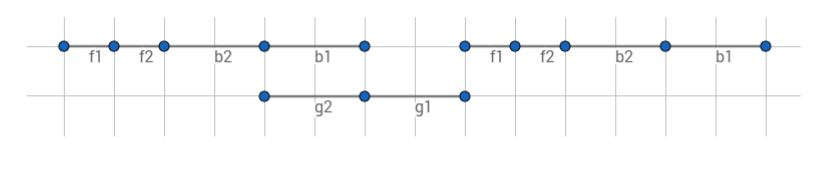
\includegraphics[scale=0.4]{figure/reducesuspend2.JPG}
	\end{figure}
\end{frame}

\begin{frame}
	\frametitle{Reduce staleness}
	\begin{figure}
		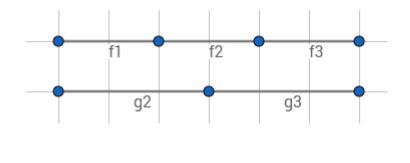
\includegraphics[scale=0.4]{figure/reducestaleness.JPG}
	\end{figure}
\end{frame}

\subsection{Problem description}
\begin{frame}
	\frametitle{Input}
	\begin{itemize}
		\item B = staleness bound.
		\item L = number of layers.
		\item I = number of iterations.
		\item W = number of workers.
		\item Cp = computation time : f1, b1, f2, b2, ...
		\item Cm = communication time : t1, t2, ...
	\end{itemize}
\end{frame}
\begin{frame}
	\frametitle{Intermediate data}
	\begin{itemize}
		\item Server maintains a set of variables indicating the minimum iteration of each layer.
		\item c1, c2, ... , cL
	\end{itemize}
\end{frame}

\begin{frame}
	\frametitle{Objective}
	\begin{itemize}
		\item Minimize training time and staleness. 
	\end{itemize}
\end{frame}

\subsection{Scheduling}
\begin{frame}
	\frametitle{Request pool}
	\begin{itemize}
		\item Pull request. 
		\item Push request. 
	\end{itemize}
\end{frame}
\begin{frame}
	\frametitle{Scheduling}
	\begin{itemize}
		\item First in first out.
		\item First in last out.
			\begin{itemize}
				\item Starvation.
			\end{itemize}
	\end{itemize}
\end{frame}
\begin{frame}
	\frametitle{Optimal solution}
	\begin{itemize}
		\item Pull
		\begin{itemize}
			\item Pull the stalest layer. 
		\end{itemize}
		\item Push
		\begin{itemize}
			\item Push the layer which can update intermediate data. 
		\end{itemize}
	\end{itemize}
\end{frame}

\section{Timetable}

\subsection{Timetable}
\begin{frame}
    \frametitle{Timetable}
	\begin{itemize}
		\item -3/31 : Finish all experiment. 
		\item -4/30 : Write paper. 
		\item 6/15- : Oral. 
	\end{itemize}
\end{frame}



\end{document}
